\documentclass[a4paper,11pt,english]{article}
\usepackage{babel}
\usepackage{ae}
\usepackage{aeguill}
\usepackage{shortvrb}
\usepackage[latin1]{inputenc}
\usepackage{tabularx}
\usepackage{longtable}
\setlength{\extrarowheight}{2pt}
\usepackage{amsmath}
\usepackage{graphicx}
\usepackage{color}
\usepackage{multirow}
\usepackage{ifthen}
\usepackage[colorlinks=false,linkcolor=black,urlcolor=black]{hyperref}
\usepackage[DIV12]{typearea}
%% generator Docutils: http://docutils.sourceforge.net/
\newlength{\admonitionwidth}
\setlength{\admonitionwidth}{0.9\textwidth}
\newlength{\docinfowidth}
\setlength{\docinfowidth}{0.9\textwidth}
\newlength{\locallinewidth}
\newcommand{\optionlistlabel}[1]{\bf #1 \hfill}
\newenvironment{optionlist}[1]
{\begin{list}{}
  {\setlength{\labelwidth}{#1}
   \setlength{\rightmargin}{1cm}
   \setlength{\leftmargin}{\rightmargin}
   \addtolength{\leftmargin}{\labelwidth}
   \addtolength{\leftmargin}{\labelsep}
   \renewcommand{\makelabel}{\optionlistlabel}}
}{\end{list}}
\newlength{\lineblockindentation}
\setlength{\lineblockindentation}{2.5em}
\newenvironment{lineblock}[1]
{\begin{list}{}
  {\setlength{\partopsep}{\parskip}
   \addtolength{\partopsep}{\baselineskip}
   \topsep0pt\itemsep0.15\baselineskip\parsep0pt
   \leftmargin#1}
 \raggedright}
{\end{list}}
% begin: floats for footnotes tweaking.
\setlength{\floatsep}{0.5em}
\setlength{\textfloatsep}{\fill}
\addtolength{\textfloatsep}{3em}
\renewcommand{\textfraction}{0.5}
\renewcommand{\topfraction}{0.5}
\renewcommand{\bottomfraction}{0.5}
\setcounter{totalnumber}{50}
\setcounter{topnumber}{50}
\setcounter{bottomnumber}{50}
% end floats for footnotes
% some commands, that could be overwritten in the style file.
\newcommand{\rubric}[1]{\subsection*{~\hfill {\it #1} \hfill ~}}
\newcommand{\titlereference}[1]{\textsl{#1}}
% end of "some commands"
\usepackage[a4paper, hmargin=2.5cm, vmargin=3cm]{geometry}
\usepackage{times}
\usepackage{nopageno}   % DON'T use page numbers!

\author {Armin Rigo
\footnote{This document has been written with the participation of Carl Friedrich Bolz (\texttt{cfbolz@gmx.de}), Holger Krekel (\texttt{hpk@merlinux.de}), Michael Hudson (\texttt{mwh@python.net}), Alex Martelli (\texttt{aleaxit@yahoo.com}) and Samuele Pedroni (\texttt{pedronis@strakt.com}).}\\
Heinrich-Heine-Universit\"at D\"usseldorf\\
\texttt{arigo@tunes.org}}
\date{}

\title{PyPy: Dynamic Optimizations for Your Favorite Language}
\hypersetup{
pdftitle={PyPy: Dynamic Optimizations for Your Favorite Language}
}
\raggedbottom
\begin{document}
\maketitle


\setlength{\locallinewidth}{\linewidth}
% command to produce latex file: 
% rst2latex.py --use-latex-citations --use-latex-footnotes --use-latex-toc --documentoptions=a4paper,11pt --hyperlink-color=0 techpaper.txt --use-latex-docinfo --stylesheet=techpaper.sty techpaper.tex 
\begin{abstract}
PyPy\footnotemark[1] is an implementation of the Python\footnotemark[2] programming language written in
Python itself, flexible and easy to experiment with.  Our long-term goals are
to target a large variety of platforms, small and large, by providing a
compiler toolsuite that can produce custom Python versions.  Platform, memory
and threading models are to become aspects of the translation process - as
opposed to encoding low level details into the language implementation itself.
Eventually, dynamic optimization techniques - implemented as another
translation aspect - should become robust against language changes.
\footnotetext[1]{
\href{http://codespeak.net/pypy}{http://codespeak.net/pypy}
}
\footnotetext[2]{
\href{http://docs.python.org/ref}{http://docs.python.org/ref}
}
\end{abstract}

%___________________________________________________________________________

\hypertarget{pypy-an-implementation-of-python-in-python}{}
\section{PyPy - an implementation of Python in Python}

It has become a tradition in the development of computer languages to
implement each language in itself.  This serves many purposes. By doing so,
you demonstrate the versatility of the language and its applicability for
large projects.  Writing compilers and interpreters are among the most
complex endeavours in software development.

An important aspect of implementing Python in Python is the high level of
abstraction and compactness of the language. This allows an implementation
that is, in some respects, easier to understand and play with than the one
written in C (referred to throughout the PyPy documentation and source as
``CPython''\footnotemark[3]).
\footnotetext[3]{
\href{http://www.python.org}{http://www.python.org}
}

Another central idea in PyPy is building the implementation in the form
of a number of independent modules with clearly defined and well tested API's. 
This eases reuse and allows experimenting with multiple implementations 
of specific features.

Later in the project we will introduce optimizations, following the
ideas of Psyco\footnotemark[4], a Just in Time Specializer, that should make PyPy
run Python programs faster than CPython. Extensions that increase the
expressive power are also planned. For instance, we will include the
ideas of Stackless\footnotemark[5], which moves the execution frames off the stack into
heap space, allowing for massive parallellism.
\footnotetext[4]{
\href{http://psyco.sourceforge.net}{http://psyco.sourceforge.net}
}
\footnotetext[5]{
\href{http://stackless.com}{http://stackless.com}
}


%___________________________________________________________________________

\hypertarget{pypy-meta-goals}{}
\section{PyPy - Meta Goals}

PyPy is not only about writing another Python interpreter.
Traditionally, interpreters are written in a target platform language
like C/Posix, Java or C{\#}.  Each such interpreter provides a ``mapping''
from application source code to the target environment.  One of the
goals of the ``all-encompassing'' environments, like the .NET framework
and to some extent the Java virtual machine, is to provide standardized
and higher level functionalities to language implementors.  This reduces
the burden of having to write and maintain many interpreters or
compilers.

PyPy is experimenting with a different approach.  We are not writing a
Python interpreter for a specific target platform.  We have written a
Python interpreter in Python, with as few references as possible to
low-level details.  (Because of the nature of Python, this is already
a complicated task, although not as complicated as writing it in - say
- C.)  Then we use this as a ``language specification'' and manipulate
it to produce the more traditional interpreters that we want.  In the
above sense, we are generating the concrete ``mappings'' of Python into
lower-level target platforms.

So far (autumn 2005), we have already succeeded in turning this ``language
specification'' into reasonably efficient C-level code that performs
basically the same job as CPython.  Memory management is inserted during
this \emph{translation} process.  It can be configured to use reference
counting or not; thus we have already achieved two very different
mappings of application Python code over C/Posix.  We have
also successfully translated our Python interpreter into LLVM\footnotemark[6] code,
and we are working on targeting higher-level environments like
Java and Squeak.

In some senses, PyPy project's central component is not its
interpreter implementation, but its configurable translator.
We think it provides a good way to avoid writing \texttt{n * m * o}
interpreters for \texttt{n} dynamic languages and \texttt{m} platforms
with \texttt{o} crucial design decisions.  PyPy aims at having any
one of these parameters changeable independently from each other:
\begin{itemize}
\item {} 
we can modify or replace the language we interpret and just regenerate
a concrete interpreter for each target;

\item {} 
we can write new translator back-ends to target new platforms;

\item {} 
we can tweak the translation process to produce low-level code based
on different models and tradeoffs.

\end{itemize}

By contrast, a standardized target environment - say .NET - 
enforces \texttt{m=1} as far as it is concerned.  This helps making \texttt{o} a
bit smaller by providing a higher-level base to build upon.  Still,
we believe that enforcing the use of one common environment 
is not necessary.  PyPy's goal is to give weight to this claim - at least 
as far as language implementation is concerned - showing an approach
to the \texttt{n * m * o} problem that does not rely on standardization.

This is the \emph{meta-goal}; a more concrete goal worth mentioning at this
point is that language specifications can be used to generate cool stuff
in addition to traditional interpreters - e.g. Just-In-Time compilers.
\footnotetext[6]{
\href{http://llvm.cs.uiuc.edu/}{http://llvm.cs.uiuc.edu/}
}


%___________________________________________________________________________

\hypertarget{higher-level-picture}{}
\section{Higher level picture}

As you would expect from a project implemented using ideas from the world
of Extreme Programming\footnotemark[7], the architecture of PyPy has evolved over time
and continues to evolve.  Nevertheless, the high level architecture is now
clear.  There are two independent basic subsystems: the Standard
Interpreter and the Translation Process.
\footnotetext[7]{
\href{http://www.extremeprogramming.com/}{http://www.extremeprogramming.com/}
}


%___________________________________________________________________________

\hypertarget{the-standard-interpreter}{}
\subsection{The Standard Interpreter}

The \emph{standard interpreter} is the subsystem implementing the Python language.
It is divided into two components:
\begin{itemize}
\item {} 
the bytecode interpreter which is responsible for interpreting 
code objects and implementing bytecodes,

\item {} 
the standard object space which implements creating, accessing and
modifying application level objects.

\end{itemize}

Note that the \emph{standard interpreter} can run fine on top of CPython if one
is willing to pay the performance penalty for double-interpretation.

The \emph{bytecode interpreter} is the part that interprets the compact
bytecode format produced from user Python sources by a preprocessing
phase, the \emph{bytecode compiler}.  The bytecode compiler itself is
implemented as a chain of flexible passes (tokenizer, lexer, parser,
abstract syntax tree builder, bytecode generator).  The bytecode
interpreter then does its work by delegating all actual manipulation of
user objects to the \emph{object space}.  The latter can be thought of as the
library of built-in types.  It defines the implementation of the user
objects, like integers and lists, as well as the operations between
them, like addition or truth-value-testing.

This division between bytecode interpreter and object space is very
important, as it gives a lot of flexibility. It is possible to use
different object spaces to get different behaviours of the Python
objects.  Using a special object space is also an important technique
for our translation process.


%___________________________________________________________________________

\hypertarget{the-translation-process}{}
\subsection{The Translation Process}

The \emph{translation process} aims at producing a different (low-level)
representation of our standard interpreter.  The \emph{translation process} 
is done in four steps:
\begin{itemize}
\item {} 
producing a \emph{flow graph} representation of the standard interpreter. 
A combination of the bytecode interpreter and a \emph{flow object space}
performs \emph{abstract interpretation} to record the flow of objects
and execution throughout a Python program into such a \emph{flow graph};

\item {} 
the \emph{annotator} which performs type inference on the flow graph;

\item {} 
the \emph{typer} which, based on the type annotations, turns the flow graph
into one using only low-level operations that fit the model of the
target platform;

\item {} 
the \emph{code generator} which translates the resulting flow graph into
another language, currently C, LLVM, Javascript (experimental).

\end{itemize}

A more complete description of the phases of this process is out of the scope
of the present introduction.  We will only give a short overview in the sequel.
\hypertarget{initialization-time}{}\hypertarget{translation-process-in-more-details}{}

%___________________________________________________________________________

\hypertarget{rpython-the-flow-object-space-and-translation}{}
\section{RPython, the Flow Object Space and translation}

One of PyPy's now achieved objectives is to enable translation of our
bytecode interpreter and standard object space into a lower-level language.
In order for our translation and type inference mechanisms to work
effectively, we need to restrict the dynamism of our interpreter-level
Python code at some point.  However, in the start-up phase, we are
completely free to use all kinds of powerful Python constructs, including
metaclasses and execution of dynamically constructed strings.  However,
when the initialization phase finishes, all code objects involved need to
adhere to a more static subset of Python:
Restricted Python, also known as RPython.

The Flow Object Space then, with the help of our bytecode interpreter,
works through those initialized RPython code objects.  The result of
this abstract interpretation is a flow graph: yet another
representation of a Python program, but one which is suitable for
applying translation and type inference techniques.  The nodes of the
graph are basic blocks consisting of Object Space operations, flowing
of values, and an exitswitch to one, two or multiple links which connect
each basic block to other basic blocks.

The flow graphs are fed as input into the Annotator.  The Annotator,
given entry point types, infers the types of values that flow through
the program variables.  This is the core of the definition of RPython:
RPython code is restricted in such a way that the
Annotator is able to infer consistent types.  How much
dynamism we allow in RPython depends on, and is restricted by, the Flow
Object Space and the Annotator implementation.  The more we can improve
this translation phase, the more dynamism we can allow.  In some cases,
however, it is more feasible and practical to just get rid
of some of the dynamism we use in our interpreter level code.  It is
mainly because of this trade-off situation that the definition of
RPython has shifted over time.  Although the Annotator is
pretty stable now and able to process the whole of PyPy, the RPython
definition will probably continue to shift marginally as we improve it.

The newest piece of this puzzle is the
\emph{Typer}, which inputs the high-level types inferred by the Annotator and
uses them to modify the flow graph in-place to replace its operations with
low-level ones, directly manipulating low-level values and data structures.

The actual low-level code is emitted by ``visiting'' the type-annotated
flow graph after the typer introduced low-level operations.  Currently we have
a C-producing backend, and an LLVM-producing backend.  The former also
accepts non-annotated or partially-annotated graphs, which allow us to
test it on a larger class of programs than what the Annotator can (or
ever will) fully process.
\begin{figure*}[htbp]\begin{center}
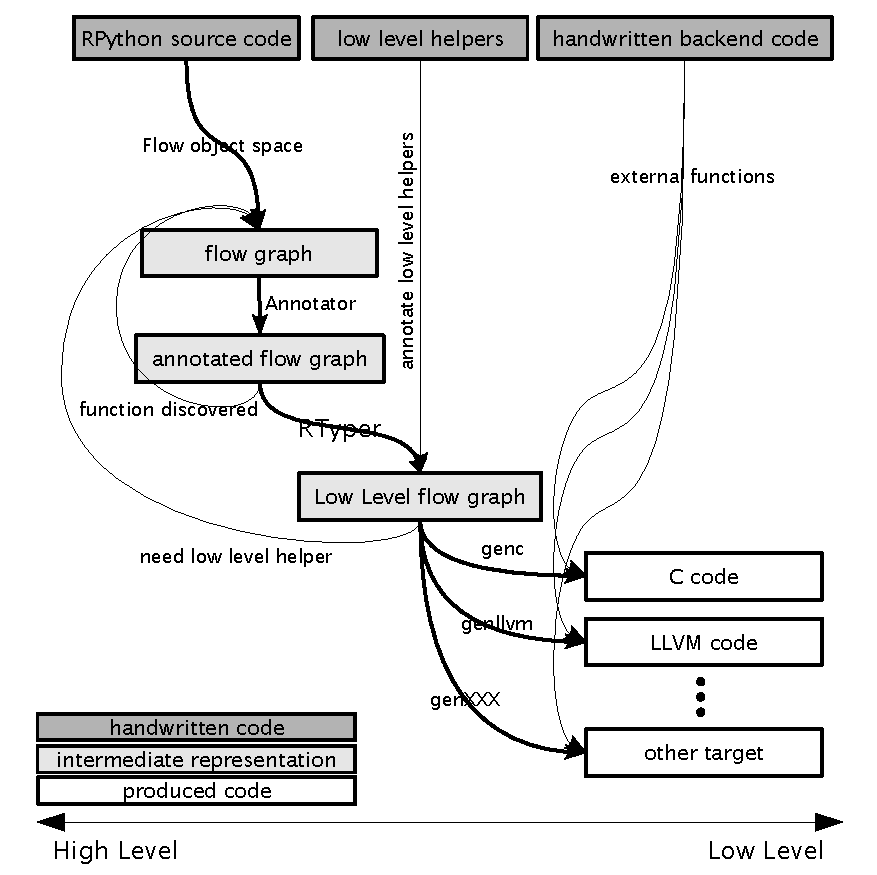
\includegraphics{translation-greyscale-small.pdf}
overview of the translation process
\end{center}\end{figure*}
The complete translation process is described in more detail in the
documentation section on the PyPy homepage\footnotemark[8].
\footnotetext[8]{
\href{http://codespeak.net/pypy}{http://codespeak.net/pypy}
}


%___________________________________________________________________________

\hypertarget{status-of-the-implementation-nov-2005}{}
\section{Status of the implementation (Nov 2005)}

With the pypy-0.8.0 release we have integrated our Abstract Syntax
Tree (AST) compiler with the rest of PyPy. The compiler gets
translated with the rest to a static self-contained version of the
standard interpreter.  Like with 0.7.0 this version is very compliant\footnotemark[9] to CPython 2.4.1 but you cannot run many existing programs on it
yet because we are still missing a number of C-modules like socket or
support for process creation.

The self-contained PyPy version (single-threaded and using the
Boehm-Demers-Weiser garbage collector\footnotemark[10]) now runs around 10-20
times slower than CPython, i.e. around 10 times faster than 0.7.0.
This is the result of optimizations, adding short cuts for some common
paths in our interpreter and adding relatively straight forward
optimising transforms to our tool chain, like inlining paired with
simple escape analysis to remove unnecessary heap allocations.  We
still have some way to go. However we expect that most of our speed
will come from the Just-In-Time compiler - work which we have barely
started yet.

With the 0.8.0 release the ``Thunk Object Space'' can also be
translated. This is a module that proxies the Standard Object Space,
adding lazy evaluation features to Python. It is a small scale
show-case for how our whole tool-chain supports flexibility from the
interpreter written in Python to the resulting self-contained
executable.

Our rather complete and Python 2.4-compliant interpreter consists 
of about 30,000-50,000 lines of code (depending on the way you
count code borrowed and adapted from other sources), with
another 14,000 lines of unit tests.  If we include the tools,
the parts related to code analysis and generation, and the
standard library modules ported from C, PyPy is now 138,000
lines of code and 32,000 lines of tests. Refer to 
the statistics web page\footnotemark[11] for more detailed information.
\footnotetext[9]{
\href{http://www.hpl.hp.com/personal/Hans_Boehm/gc/}{http://www.hpl.hp.com/personal/Hans{\_}Boehm/gc/}
}
\footnotetext[10]{
\href{http://codespeak.net/~hpk/pypy-testresult/}{http://codespeak.net/{\textasciitilde}hpk/pypy-testresult/}
}
\footnotetext[11]{
\href{http://codespeak.net/~hpk/pypy-stat/}{http://codespeak.net/{\textasciitilde}hpk/pypy-stat/}
}


%___________________________________________________________________________

\hypertarget{future-work-and-foreseen-possibilities}{}
\section{Future work and foreseen possibilities}

In 2006, the PyPy project aims to translate the standard Python
Interpreter to a JIT-compiler and also to support massive parallelism
(micro-threads) within the language.  These are not trivial tasks
especially if we want to retain and improve the modularity and
flexibility aspects of our implementation - like giving an independent
choice of memory or threading models for translation.  Moreover it is
likely that our Javascript and other higher level backends (in
contrast to our current low-level ones) will continue to evolve.

Apart from optimization-related translation choices PyPy is to enable
new possibilities regarding persistence, security and distribution
issues.  We intend to experiment with ortoghonal persistence for
Python objects, i.e. one that doesn't require application objects to
behave in a particular manner.  Security-wise we will look at
sandboxing or capabilities based schemes.  For distribution we already
experimented with allowing transparent migration of objects between
processes with the help of the existing (and translateable) Thunk
Object Space.  In general, all experiments are much easier to conduct
in PyPy and should provide a resulting standalone executable in
a shorter time than traditional approaches.

\end{document}
